\documentclass[lettersize,journal]{IEEEtran}
\usepackage{amsmath,amsfonts}
\usepackage{algorithmic}
\usepackage{algorithm}
\usepackage{array}
\usepackage[caption=false,font=normalsize,labelfont=sf,textfont=sf]{subfig}
\usepackage{textcomp}
\usepackage{stfloats}
\usepackage{url}
\usepackage{verbatim}
\usepackage{graphicx}
\usepackage{cite}
\usepackage{tikz}
\usepackage{hyperref}

\begin{document}

    \title{Binary Serialization of an Intermediate Representation\\SASPS}

    \author{Ștefan Silviu-Alexandru,~\IEEEmembership{SSA-2,\\~Faculty of Computers and Automatic Control, University POLITEHNICA of Bucharest}}

    \maketitle

%    \begin{abstract}
%        Abstract abstract abstract abstract abstract abstract abstract abstract abstract abstract :)
%    \end{abstract}

    \section{Introduction}\label{sec:introduction}

    \IEEEPARstart{T}{his} document analyzes the performance of binary serialization of a C compiler's intermediate
    representation (IR).
    In particular, we will measure and optimize how CKompiler's~\cite{ckompiler-github} IR is serialized to its binary
    form, and then deserialized back into the existing in-memory representation as Java Virtual Machine (JVM) objects.

    CKompiler was my diploma project~\cite{ckompiler}, and consists of two main components:
    a C compiler, and a method for exploring internal representations of the code inside the compiler, with interactive
    visualizations for some algorithms in the compiler.

    The IR is part of the compiler itself, and sits in the so-called "middle-end", after the lexical analysis, parsing,
    and semantic analysis of the frontend, but before any code generation or target-specific transformations.

    \subsection{Purpose of Serializing IR}\label{subsec:purpose-of-serializing-ir}

    There are a few benefits to having the ability to serialize IR:
    \begin{itemize}
        \item Interoperability.
        Other programs could then theoretically read and write IR files, for example to perform static analysis.
        \item Further decoupling the frontend from the backend.
        For example, another program could parse a different language from C, generate a serialized IR file, then send
        it to CKompiler's backend for assembly generation.
        \item Testing.
        Currently, due to convenience, most of CKompiler's automated tests for code generation pass C code through
        the parser and other steps in order to generate the test IR\@.
        With serialized IR files, the test data can be controlled completely, avoiding situations where a bug in the
        parser or the IR generation causes unrelated code generation tests to fail.
    \end{itemize}

    Better known compiler projects such as LLVM also support a binary serialized form of their IR, the LLVM bitcode
    representation~\cite{llvm,llvm-ir}.

    A binary format is chosen over a text format because the CKompiler IR is not meant to be human-readable, instead
    relying on being efficiently processed by tools.
    Using a binary format also helps with keeping file size down.

    \subsection{Objectives}\label{subsec:objectives}

    First, the implementation of a serializer and a deserializer must be created.
    While the IR exists and is (relatively) stable, it currently resides in memory, and was not intended for anything
    more.
    The implementation is described in section~\ref{sec:implementation-details}.

    With an initial implementation done, a benchmark suite can then be developed, for both CPU time and memory.
    Details about the methodology and the content of the test suite are in section~\ref{sec:methodology}.

    Then, the implementation can be optimized, and the benchmark executed again.
    The results from the benchmark runs are presented and discussed in section~\ref{sec:results}.

    \section{Implementation Details}\label{sec:implementation-details}

    The focus is on serializing Control Flow Graphs (CFGs) for individual functions.
    In CKompiler, this structure includes all the IR for each basic block in the graph, the control flow represented
    as edges between the basic blocks, and the $\phi$ functions for each basic block that contains variable join points.

    CKompiler's IR is in three-address form, and the IR values respect the Static Single Assignment (SSA) property.
    There are two primary class hierarchies involved in representing the IR, described in
    sections~\ref{subsec:ir-value-hierarchy} and~\ref{subsec:ir-instruction-hierarchy}.

    The serializers and deserializers themselves were implemented using Kotlin's official serialization
    library~\cite{kotlinx-serialization, kotlinx-serialization-git} (see~\ref{subsec:kotlinx-serialization}).

    \subsection{Kotlin Serialization}\label{subsec:kotlinx-serialization}

    \texttt{kotlinx.serialization} is an annotation-based serialization library.
    Adding the \texttt{@Serializable} annotation to a class automatically generates a descriptor that lists every
    field that must be serialized and deserialized.
    Based on the descriptor, the serializer can convert an instance to the selected format, and the deserializer can do
    the inverse.

    Other annotations that were used are:
    \begin{itemize}
        \item \texttt{@SerialName}, which can resolve name conflicts;
        \item \texttt{@Transient}, which skips a particular field from serialization when its value can simply be
        computed from the other fields;
        \item {\small\texttt{@Serializable(with~=~SomeSerializer::class)},\par} which instead of auto-generating the descriptor,
        uses a handwritten one for special cases.
    \end{itemize}

    The library offers support for JSON (among others), but for this binary format we will have to implement custom
    logic.
    This is achieved by implementing the \texttt{Decoder} and \texttt{Encoder} interfaces, as outlined in the
    documentation~\cite{kotlinx-serialization-custom-format}.

    The implementations of the two interfaces makes use of \texttt{java.io.DataInput} and \texttt{java.io.DataOutput},
    respectively, to read and write primitives as bytes.

    Additionally, a signature is prepended to the serialized data.
    Adding a couple of unprintable bytes ensures the file is not mistaken for a text file, the string "CKI IR" makes it
    easy to recognize the file type, and the format revision allows rejecting incompatible versions of the format.

    \begin{footnotesize}
        \begin{verbatim}
val binarySerializationSignature = ubyteArrayOf(
    0x01u, 0xFFu,
    *"CKI IR".encodeToByteArray().toUByteArray(),
    binaryFormatRevision
)
        \end{verbatim}
    \end{footnotesize}

    \subsection{IR Value Hierarchy}\label{subsec:ir-value-hierarchy}

    The values in the IR represent all the various elements expected of a program:

    \begin{itemize}
        \item variables and temporaries;
        \item string, float, integer and other constants;
        \item memory references;
        \item fixed register references.
    \end{itemize}

    \begin{figure}[th]
        \centering
        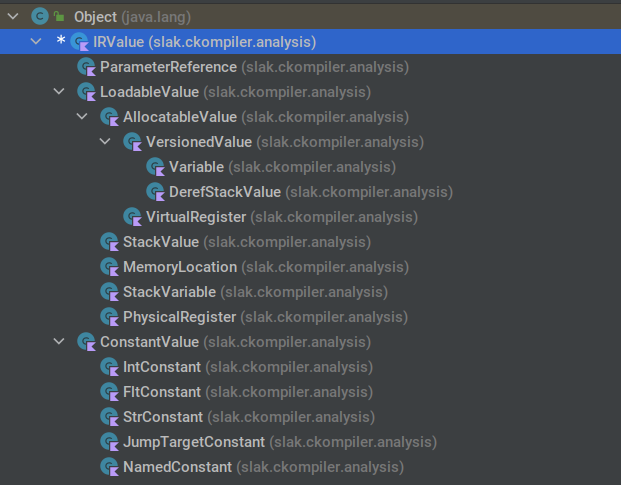
\includegraphics[width=0.45\textwidth]{pics/irvalue-hierarchy}
        \caption{Class hierarchy of \texttt{IRValue}}
        \label{fig:irvalue-hierarchy}
    \end{figure}

    The complete hierarchy is in figure~\ref{fig:irvalue-hierarchy}.
    Preparing the values themselves for serialization is not difficult.
    For variables and temporaries, it is sufficient to store their unique ID, their name, and their type.
    For constants, the actual value along with its type is enough.
    Finally, for various references the kind of reference and the referenced ID are stored.

    The only challenge here was in the types, as the type system representation in CKompiler is insufficiently
    abstract, and contains irrelevant information for the IR\@.
    By converting some fields to computed properties, and excluding others from serialization using the
    \texttt{@Transient} annotation (see~\ref{subsec:kotlinx-serialization}), the types were serialized and deserialized
    successfully.

    \subsection{IR Instruction Hierarchy}\label{subsec:ir-instruction-hierarchy}

    The instruction set itself, in figure~\ref{fig:irinstruction-hierarchy}, is actually quite small.
    Most of the fields in such an instruction are \texttt{IRValue}s, which make the instructions easy to serialize.

    \begin{figure}[th]
        \centering
        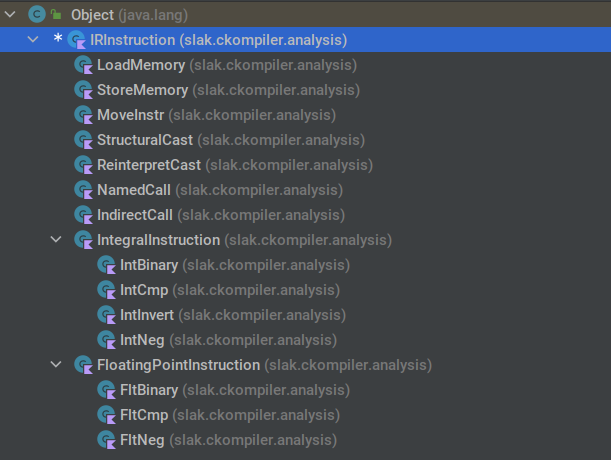
\includegraphics[width=0.45\textwidth]{pics/irinstruction-hierarchy}
        \caption{Class hierarchy of \texttt{IRInstruction}}
        \label{fig:irinstruction-hierarchy}
    \end{figure}

    \subsection{CFG and Basic Blocks}\label{subsec:cfg-and-basic-blocks}

    The remaining classes to serialize are those that make up the graph itself:
    \begin{itemize}
        \item \texttt{CFG}, which acts as a container for everything else
        \item \texttt{BasicBlock}, a node in the control flow graph, which is identified using a unique ID
        \item \texttt{Jump} and its subclasses, which represents CFG edges, linking \texttt{BasicBlock}s
    \end{itemize}

    There are a few challenges intrinsic to this kind of graph representation.

    First, the graph is maintained as an actual graph of references in memory, with the CFG holding references to nodes,
    and the nodes holding references to predecessor/successor nodes.
    Since control flow graphs for programs are almost guaranteed to contain cycles (for loops and while loops become
    cycles in the program CFG), it implies there are cyclical references between the nodes and the edges instances.
    Of course, this is impossible to serialize as-is.

    The solution in this case is to rely on the unique IDs of each \texttt{BasicBlock}, and replace all references with
    the ID of the referenced object.
    The blocks are serialized only once, in a list that contains all \texttt{BasicBlock}s, so the deserialization
    process can do the inverse mapping, and recreate the references from the IDs and this list.

    A related issue during deserialization is the need to create all the \texttt{BasicBlock}s upfront, to deal
    with the cyclical references.
    This is analogous to the process with which the CFG is created in the first place, where the blocks are created
    first, and only later linked with one another.

    Another issue related to this ID mapping is thread safety.
    CKompiler is designed to have the ability to process compilation units in parallel, which means certain processes
    must be atomic, or the state they rely on must not be global.
    In order to retain this useful property for the deserialization process, and permit parallel deserialization, care
    must be taken to keep the ID mapping in thread-local variables.

    A different issue was the way in which the CFG object itself was constructed.
    Originally, the constructor for the CFG class received a parsed function, and internally executed the code that
    converts that function to a CFG instance.
    This is a problem for deserialization, as none of that code should run when creating the CFG from serialized IR\@.

    To resolve the issue, the \texttt{CFGFactory} class was introduced.
    All the work previously done in the constructor is now part of the factory, and any options are passed directly to
    the factory, like the example in figure~\ref{fig:cfg-factory-create}.
    The original \texttt{CFG} class has been converted into a plain data class, which contains no logic or methods,
    only the result of converting a function to a control flow graph.
    As a result, there are two avenues for obtaining a CFG instance; the factory and the deserializer, the latter
    bypassing the factory to create a CFG instance directly.

    \begin{figure}[th]
        \centering
        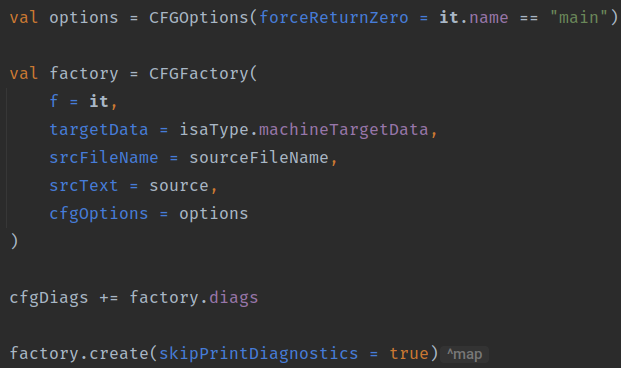
\includegraphics[width=0.45\textwidth]{pics/cfgfactory}
        \caption{Using \texttt{CFGFactory} to create a CFG instance}
        \label{fig:cfg-factory-create}
    \end{figure}

    The final issue is related to debugging information.
    Many of these classes contain referenced to the parser output, which in turn contains references to where in the
    source text the IR originates from.
    The solution is to omit this debug data from the serialized format, and eventually output it separately,
    perhaps using a widespread standard such as DWARF~\cite{dwarf-standard}.

    \section{Optimizations}\label{sub:optimizations}

    After the initial implementation, several optimizations are implemented to reduce both CPU usage and memory
    allocations, and they are discussed below.

    \subsection{Flyweight}\label{subsec:flyweight}

    The main optimization is the use of the Flyweight design pattern.
    Several classes inside the compiler are well suited to being cached and shared in this manner.
    Section~\ref{sec:results} shows how the pattern not only reduces allocations, but also CPU usage, because allocating
    and then deallocating so much memory takes a measurable amount of time.

    We can now look at an example where Flyweight was used.
    The ~\texttt{Variable} class contains immutable information that is shared by many instances.
    A "variable" in a C program has three important attributes, its name, its type, and its scope.
    Scoping is handled by the parser, and is of no concern to the IR\@.
    Due to name shadowing, a variable's name is not unique.
    To discriminate between shadowed variables, a unique ID is assigned to each variable, making sure they are not equal
    even if they happen to have the same name.

    All of this information is immutable, and a variable's ID, name, and type do not change.
    This would allow the same variable instance to be shared everywhere that variable is referenced.
    However, the \texttt{Variable} class represents variables as determined by the Static Single Assignment (SSA) form,
    not variables in the C sense.

    SSA is a key part of modern compilers, because its properties greatly simplify several optimizations and
    transformations that are applied to the code before code generation.
    The "Single Assignment" part requires that each variable is assigned to only once, which clearly doesn't fit with
    the mutable-by-default C variables.
    Conversion to SSA form includes a process called "variable renaming", where each new assignment to a variable
    is converted to assignment of a new, different variable, and future uses updated to match this new variable.

    A string of code such as \texttt{int a = 1; f(a); a = 2; f(a);} would be converted to
    \texttt{int a\textsubscript{1} = 1; f(a\textsubscript{1}); a\textsubscript{2} = 2; f(a\textsubscript{2});}.
    Now, even though all references have the same type ("int"), the same ID, and used to refer to the same variable
    name ("a"), they each have different versions ("a\textsubscript{1}" and "a\textsubscript{2}").
    The existing implementation in CKompiler was naive, and resulted in not just duplication of all the data for each
    variable, but duplication of it for every version of every variable.

    As a result, in this string of code there would be 4 \texttt{Variable} instances, with 4 copies of the ID, 4 copies
    of the name and 4 references to the integer type, which is suboptimal.

    To resolve the issue, a Flyweight Factory was introduced (\texttt{IRValueFactory}).
    This class caches \texttt{TypedIdentifier} instances, which encapsulate the shared state mentioned above
    (ID, name, type).
    Now, when the factory is used to create a \texttt{Variable}, only the version and a referenced to the cached
    \texttt{TypedIdentifier} are stored in the \texttt{Variable} instance.

    When serializing, the cache is stored as part of the binary data.
    Instead of having to read the same name and type again and again, the deserialization process only has to read a
    single 4 byte cache key.
    Since initially the pointers to the name and the type were 8 bytes each, the savings are good without even counting
    the referenced data itself.

    The Flyweight pattern was also applied to \texttt{BasicBlock} and integer constants in a similar manner.
    There are still candidates for future improvements using this pattern, such as the objects used to represent struct
    and union types, or some other constants.

    \subsection{Miscellaneous Optimizations}\label{subsec:miscellaneous-optimizations}

    While benchmarking the code and implementing Flyweight, other opportunities for optimization were taken.

    First, a reduction in the size of serialized class names.
    To serialize a list of polymorphic classes, each object of the list must be prefixed with an identifier for the
    class, to know which concrete subclass it should deserialize into.
    By default, this identifier is the fully qualified name, which is long.
    It is now replaced with unique single-byte identifiers.
    This incidentally reduced the size of the serialized code by several MB in the worst cases.

    Second, the in-memory and serialized format of some stored data was unified.
    This way, serialization doesn't have to convert from in-memory to serialized, and deserialization doesn't have to do
    the reverse, because the format is the same.

    And finally, the implementation of \texttt{IRDecoder} recursively instantiated itself to decode lists of objects,
    which caused memory churn in nested lists.
    By moving to a non-recursive implementation that uses a stack, the churn was minimized.

    \section{Measurement Methodology}\label{sec:methodology}

    To evaluate the effect of the optimizations on the serialization and deserialization process, a set of
    benchmarks was developed.
    The primary measurements are average CPU time and memory allocations.

    \subsection{Benchmarking Suite}\label{subsec:benchmarking-suite}

    CKompiler is written in Kotlin, and the main execution environment is the JVM, which means the Java Microbenchmark
    Harness (JMH) is available.
    JMH is an OpenJDK project~\cite{jmh-github}, and provides an automated method of benchmarking performance of JVM
    code.
    While JMH was intended for Java code, it is possible to use it for Kotlin code via a
    library~\cite{kotlinx-benchmark}.

    Simply measuring the time taken by the execution is incorrect for Just In Time (JIT) compiled runtimes, of which the
    JVM is an example.
    This is the case since the compilation time affects the results, and the garbage collector stop-the-world pauses can
    skew the results.
    JMH already contains ways to mitigate or remove these extraneous variables, so there is no need to reinvent the
    wheel, when a standard tool is available.

    \subsection{Tiered compilation}\label{subsec:tiered-compilation}

    Additionally, OpenJDK employs tiered compilation~\cite{tiered-compilation}, and to get reproducible results we need
    to use the same compiler for all tests.
    OpenJDK's runtime contains an initial interpreter, a first tier fast compiler (C1), and a second tier optimizing
    compiler (C2).
    It is a fairly standard tiered compilation architecture, found in other similar language runtimes such as
    Chromium's V8 runtime for JavaScript~\cite{v8-tiered}.

    This is an aspect that JMH helps with.
    By executing the benchmark code several times in a "warmup" routine, it forces the runtime into always optimizing
    the code through C2 before capturing the real benchmark results.

    For example, here's an example of the initial warmup iteration output, for an instance of the deserialization
    benchmark:
    \begin{verbatim}
# Warmup Iteration   1: 0.492 ms/op
# Warmup Iteration   2: 0.418 ms/op
# Warmup Iteration   3: 0.414 ms/op
# Warmup Iteration   4: 0.400 ms/op
# Warmup Iteration   5: 0.399 ms/op
    \end{verbatim}

    This illustrates the issues with tiered compilation mentioned above.
    The first iteration is the slowest of them all, the second and third are faster, and the final two are the fastest.
    The test runs of this example, that follow the warmup iterations generated values around 0.400 ms/op, with errors of
    at most 0.010 ms/op, making them quite similar to the last two warmup iterations.
    This is a confirmation that the benchmark code has been optimized by the highest performing compiler of the runtime.
    If the value were to continue to fluctuate, it would be a sign that something in the benchmark setup was incorrect.

    \subsection{Interpreting JMH Results}\label{subsec:interpreting-jmh-results}

    An example of all the metrics tracked by JMH with the GC profiler enabled is present in
    table~\ref{tab:jmh-example}.

    \begin{table*}[t]
        \centering
        \begin{tabular}{l l l r l r}
            Benchmark                                    & Mode & Cnt  &     Score &        Error &   Units \\
            example                                      & avgt &  10  &    16.060 & ±      0.677 &   ms/op \\
            example:·gc.alloc.rate                       & avgt &  10  &     2.850 & ±      0.124 &  MB/sec \\
            example:·gc.alloc.rate.norm                  & avgt &  10  & 71770.146 & ±    264.912 &    B/op \\
            example:·gc.churn.G1\_Eden\_Space            & avgt &  10  &     3.447 & ±     11.032 &  MB/sec \\
            example:·gc.churn.G1\_Eden\_Space.norm       & avgt &  10  & 85320.030 & ± 273386.799 &    B/op \\
            example:·gc.churn.G1\_Survivor\_Space        & avgt &  10  &     0.003 & ±      0.014 &  MB/sec \\
            example:·gc.churn.G1\_Survivor\_Space.norm   & avgt &  10  &    73.841 & ±    353.029 &    B/op \\
            example:·gc.count                            & avgt &  10  &     2.000 &              &  counts \\
            example:·gc.time                             & avgt &  10  &     3.000 &              &      ms \\
        \vspace{2pt}
        \end{tabular}
        \caption{An example of the metrics collected by JMH and the GC profiler}
        \label{tab:jmh-example}
    \end{table*}

    The first relevant metric is the CPU time taken by the benchmarked code, and it is the first in the list.
    In this example, it is $\sim$16 ms/op, with an error of $\sim$0.7 ms/op, which means all results
    are within $\sim$5\% of the average.

    The second relevant metric is the normalized allocation rate, the third in the list (\texttt{gc.alloc.rate.norm}).
    In other words, how much memory was allocated every benchmark iteration.
    This particular metric hides variance related to when the garbage collector runs, how often it runs, or even which
    kind of GC is used.
    In this example, the value is $\sim$72 kB/op, with an error of $\sim$264 B/op, which is just
    under 0.4\%.

    The remaining numbers are mostly useful for validation.

    \texttt{gc.count} and \texttt{gc.time}, for example, reveal how many times the GC was executed, and how long the
    GC takes on average.
    In this example, there were only two GC executions, whose execution lasted three milliseconds, which is negligible.
    If the benchmark code was misbehaving with respect to memory usage, a longer GC duration and increased GC counts
    would have been observed.

    The G1-related metrics are specific to the G1 garbage collector, the default of the JVM\@.
    G1 is a generational GC, like many other JVM GC implementations, and the metrics track memory churn through its
    generations: the young generation, named "Eden Space", and the old generation, named "Survivor Space".
    If there was a memory leak in the benchmark, preserving references between benchmark iterations and invalidating the
    allocation results, there might be a visible and proportional increase in the
    \texttt{gc.churn.G1\_Survivor\_Space.norm} metric, which sits at merely $\sim$74 B/op in this example, a
    negligible amount of memory.

    \section{Results}\label{sec:results}

    The benchmark discussed in section~\ref{sec:methodology} was applied to four inputs.
    Both serialization and deserialization was tested for each of them.

    The percentages in the following sections are rounded to the nearest integer, and the raw numbers from the tables
    are converted to more readable units (kB, MB, etc) and truncated to 1 significant digit.

    \subsection{Empty Function}\label{subsec:empty-function}

    The first input was simply an empty function.
    This test establishes a lower boundary for both serialization and deserialization.
    It also serves to check how large the fixed cost of serialization and deserialization is.

    Tables~\ref{tab:initial-empty} and~\ref{tab:final-empty} show benchmark results before and after the optimizations,
    respectively.

    The allocation rate for serialization is mostly unchanged, at around 5kB per serialization.
    For deserialization, there was a minor 11\% improvement, from 8.7kB to 7.7kB\@.

    The CPU usage is extremely low, and both serialization and deserialization take under 3000ns per operation,
    which is essentially zero when compared to serialization time for real programs.

    \begin{table*}[t]
        \centering
        \begin{tabular}{l l l r l r}
            Benchmark                                                     & Mode & Cnt &     Score    &        Error  &  Units \\
            serializeEmpty                                                & avgt &  20 &     2167.662 & ±      37.712 &  ns/op \\
            serializeEmpty:·gc.alloc.rate                                 & avgt &  20 &     1537.137 & ±      25.753 & MB/sec \\
            serializeEmpty:·gc.alloc.rate.norm                            & avgt &  20 &     5240.119 & ±       0.015 &   B/op \\
            serializeEmpty:·gc.churn.G1\_Eden\_Space                      & avgt &  20 &     1522.672 & ±     193.803 & MB/sec \\
            serializeEmpty:·gc.churn.G1\_Eden\_Space.norm                 & avgt &  20 &     5193.181 & ±     670.769 &   B/op \\
            serializeEmpty:·gc.churn.G1\_Survivor\_Space                  & avgt &  20 &        0.003 & ±       0.002 & MB/sec \\
            serializeEmpty:·gc.churn.G1\_Survivor\_Space.norm             & avgt &  20 &        0.009 & ±       0.008 &   B/op \\
            serializeEmpty:·gc.count                                      & avgt &  20 &       42.000 &               & counts \\
            serializeEmpty:·gc.time                                       & avgt &  20 &       19.000 &               &     ms \\
            \\
            deserializeEmpty                                              & avgt &  20 &     2645.413 & ±      51.571 &  ns/op \\
            deserializeEmpty:·gc.alloc.rate                               & avgt &  20 &     2100.118 & ±      40.917 & MB/sec \\
            deserializeEmpty:·gc.alloc.rate.norm                          & avgt &  20 &     8736.216 & ±       0.023 &   B/op \\
            deserializeEmpty:·gc.churn.G1\_Eden\_Space                    & avgt &  20 &     2115.540 & ±     235.591 & MB/sec \\
            deserializeEmpty:·gc.churn.G1\_Eden\_Space.norm               & avgt &  20 &     8803.532 & ±     986.388 &   B/op \\
            deserializeEmpty:·gc.churn.G1\_Survivor\_Space                & avgt &  20 &        0.003 & ±       0.002 & MB/sec \\
            deserializeEmpty:·gc.churn.G1\_Survivor\_Space.norm           & avgt &  20 &        0.011 & ±       0.009 &   B/op \\
            deserializeEmpty:·gc.count                                    & avgt &  20 &       64.000 &               & counts \\
            deserializeEmpty:·gc.time                                     & avgt &  20 &       28.000 &               &     ms \\
        \vspace{2pt}
        \end{tabular}
        \caption{Initial results for an empty function}
        \label{tab:initial-empty}
    \end{table*}

    \begin{table*}[t]
        \centering
        \begin{tabular}{l l l r l r}
            Benchmark                                                     & Mode & Cnt &     Score    &         Error  &  Units \\
            serializeEmpty                                                & avgt &  20 &     2050.538 & ±       36.301 &   ns/op \\
            serializeEmpty:·gc.alloc.rate                                 & avgt &  20 &     1590.259 & ±       27.311 &  MB/sec \\
            serializeEmpty:·gc.alloc.rate.norm                            & avgt &  20 &     5128.126 & ±        0.021 &    B/op \\
            serializeEmpty:·gc.churn.G1\_Eden\_Space                      & avgt &  20 &     1580.550 & ±      285.946 &  MB/sec \\
            serializeEmpty:·gc.churn.G1\_Eden\_Space.norm                 & avgt &  20 &     5093.301 & ±      900.706 &    B/op \\
            serializeEmpty:·gc.churn.G1\_Survivor\_Space                  & avgt &  20 &        0.002 & ±        0.002 &  MB/sec \\
            serializeEmpty:·gc.churn.G1\_Survivor\_Space.norm             & avgt &  20 &        0.007 & ±        0.006 &    B/op \\
            serializeEmpty:·gc.count                                      & avgt &  20 &       49.000 &                &  counts \\
            serializeEmpty:·gc.time                                       & avgt &  20 &       21.000 &                &      ms \\
            \\
            deserializeEmpty                                              & avgt &  20 &     2930.053 & ±       33.954 &   ns/op \\
            deserializeEmpty:·gc.alloc.rate                               & avgt &  20 &     1685.482 & ±       19.228 &  MB/sec \\
            deserializeEmpty:·gc.alloc.rate.norm                          & avgt &  20 &     7768.198 & ±        0.028 &    B/op \\
            deserializeEmpty:·gc.churn.G1\_Eden\_Space                    & avgt &  20 &     1684.230 & ±      254.690 &  MB/sec \\
            deserializeEmpty:·gc.churn.G1\_Eden\_Space.norm               & avgt &  20 &     7758.977 & ±     1156.194 &    B/op \\
            deserializeEmpty:·gc.churn.G1\_Survivor\_Space                & avgt &  20 &        0.002 & ±        0.002 &  MB/sec \\
            deserializeEmpty:·gc.churn.G1\_Survivor\_Space.norm           & avgt &  20 &        0.009 & ±        0.009 &    B/op \\
            deserializeEmpty:·gc.count                                    & avgt &  20 &       54.000 &                &  counts \\
            deserializeEmpty:·gc.time                                     & avgt &  20 &       22.000 &                &      ms \\
        \vspace{2pt}
        \end{tabular}
        \caption{Final results for an empty function}
        \label{tab:final-empty}
    \end{table*}

    \subsection{Hello World Function}\label{subsec:hello-world-function}

    This test is another synthetic test, which contains a function that repeatedly calls printf hundreds of times:
    \texttt{printf("Hello World!\textbackslash{}n");}.
    It is essentially the worst case for this Flyweight implementation, where there are no variables to deduplicate
    (except the printf function itself).
    The string is interned by the JVM, so it should not affect allocations.

    Tables~\ref{tab:initial-hello-world} and~\ref{tab:final-hello-world} show benchmark results before and after the
    optimizations, respectively.

    Still, there are some measurable improvements.
    Serialization time improved by 24\%, while deserialization only by 8\%.
    Memory allocation rate dropped significantly.
    For serialization, from 3.1MB to 1.6MB (46\%), and for deserialization from 3.4MB to 2MB (42\%).
    The corresponding decrease in GC count supports this result, as the lower allocation rate creates less garbage to
    collect.

    \begin{table*}[t]
        \centering
        \begin{tabular}{l l l r l r}
            Benchmark                                                     & Mode & Cnt &     Score    &        Error  &  Units \\
            serializeHelloWorld                                           & avgt &  20 &        1.694 & ±       0.023 &  ms/op \\
            serializeHelloWorld:·gc.alloc.rate                            & avgt &  20 &     1170.154 & ±      15.149 & MB/sec \\
            serializeHelloWorld:·gc.alloc.rate.norm                       & avgt &  20 &  3116886.757 & ±      15.813 &   B/op \\
            serializeHelloWorld:·gc.churn.G1\_Eden\_Space                 & avgt &  20 &     1193.449 & ±     263.126 & MB/sec \\
            serializeHelloWorld:·gc.churn.G1\_Eden\_Space.norm            & avgt &  20 &  3178120.830 & ±  698505.782 &   B/op \\
            serializeHelloWorld:·gc.churn.G1\_Survivor\_Space             & avgt &  20 &        0.236 & ±       0.102 & MB/sec \\
            serializeHelloWorld:·gc.churn.G1\_Survivor\_Space.norm        & avgt &  20 &      629.355 & ±     272.054 &   B/op \\
            serializeHelloWorld:·gc.count                                 & avgt &  20 &       35.000 &               & counts \\
            serializeHelloWorld:·gc.time                                  & avgt &  20 &       20.000 &               &     ms \\
            \\
            deserializeHelloWorld                                         & avgt &  20 &        1.794 & ±       0.014 &  ms/op \\
            deserializeHelloWorld:·gc.alloc.rate                          & avgt &  20 &     1239.554 & ±       9.321 & MB/sec \\
            deserializeHelloWorld:·gc.alloc.rate.norm                     & avgt &  20 &  3497638.988 & ±      17.302 &   B/op \\
            deserializeHelloWorld:·gc.churn.G1\_Eden\_Space               & avgt &  20 &     1216.646 & ±     268.257 & MB/sec \\
            deserializeHelloWorld:·gc.churn.G1\_Eden\_Space.norm          & avgt &  20 &  3435763.581 & ±  763881.430 &   B/op \\
            deserializeHelloWorld:·gc.churn.G1\_Survivor\_Space           & avgt &  20 &        0.161 & ±       0.086 & MB/sec \\
            deserializeHelloWorld:·gc.churn.G1\_Survivor\_Space.norm      & avgt &  20 &      453.136 & ±     242.430 &   B/op \\
            deserializeHelloWorld:·gc.count                               & avgt &  20 &       35.000 &               & counts \\
            deserializeHelloWorld:·gc.time                                & avgt &  20 &       21.000 &               &     ms \\
        \vspace{2pt}
        \end{tabular}
        \caption{Initial results for a function with repeating Hello World}
        \label{tab:initial-hello-world}
    \end{table*}

    \begin{table*}[t]
        \centering
        \begin{tabular}{l l l r l r}
            Benchmark                                                     & Mode & Cnt &     Score    &         Error  &  Units \\
            serializeHelloWorld                                           & avgt & 20  &       1.283  & ±        0.027 &  ms/op \\
            serializeHelloWorld:·gc.alloc.rate                            & avgt & 20  &     832.852  & ±       17.469 & MB/sec \\
            serializeHelloWorld:·gc.alloc.rate.norm                       & avgt & 20  & 1679884.748  & ±       14.606 &   B/op \\
            serializeHelloWorld:·gc.churn.G1\_Eden\_Space                 & avgt & 20  &     818.933  & ±      258.886 & MB/sec \\
            serializeHelloWorld:·gc.churn.G1\_Eden\_Space.norm            & avgt & 20  & 1650102.077  & ±   515598.743 &   B/op \\
            serializeHelloWorld:·gc.churn.G1\_Survivor\_Space             & avgt & 20  &       1.235  & ±        3.739 & MB/sec \\
            serializeHelloWorld:·gc.churn.G1\_Survivor\_Space.norm        & avgt & 20  &    2578.110  & ±     7847.091 &   B/op \\
            serializeHelloWorld:·gc.count                                 & avgt & 20  &      27.000  &                & counts \\
            serializeHelloWorld:·gc.time                                  & avgt & 20  &      20.000  &                &     ms \\
            \\
            deserializeHelloWorld                                         & avgt & 20  &       1.654  & ±        0.024 &  ms/op \\
            deserializeHelloWorld:·gc.alloc.rate                          & avgt & 20  &     780.818  & ±       11.288 & MB/sec \\
            deserializeHelloWorld:·gc.alloc.rate.norm                     & avgt & 20  & 2030813.501  & ±       15.869 &   B/op \\
            deserializeHelloWorld:·gc.churn.G1\_Eden\_Space               & avgt & 20  &     773.202  & ±      227.350 & MB/sec \\
            deserializeHelloWorld:·gc.churn.G1\_Eden\_Space.norm          & avgt & 20  & 2016814.460  & ±   613234.053 &   B/op \\
            deserializeHelloWorld:·gc.churn.G1\_Survivor\_Space           & avgt & 20  &       1.324  & ±        3.836 & MB/sec \\
            deserializeHelloWorld:·gc.churn.G1\_Survivor\_Space.norm      & avgt & 20  &    3462.174  & ±    10048.728 &   B/op \\
            deserializeHelloWorld:·gc.count                               & avgt & 20  &      24.000  &                & counts \\
            deserializeHelloWorld:·gc.time                                & avgt & 20  &      30.000  &                &     ms \\
        \vspace{2pt}
        \end{tabular}
        \caption{Final results for a function with repeating Hello World}
        \label{tab:final-hello-world}
    \end{table*}

    \subsection{Randomly Generated Function}\label{subsec:randomly-generated-function}

    This test consists of a function whose CFG was generated at random.
    The random C program generator adds if-else, for and while structures.
    It randomizes placement, nesting, the expressions, variables and values inside.

    Here's a representative example:
    \begin{verbatim}
if (24 >= 0) {
  while (-105 != 0) {
    res3 = array[135];
    // this is a random comment!
    array[56] = 53;
    // this is a random comment!
  }
} else {
  for (i = 0; i < 14; i = i + 1) {
    res28 = res1 * -111;
    res7 = array[106];
    // this is a random comment!
    array[139] = 26;
    // this is a random comment!
  }
}
    \end{verbatim}

    This provides a great stress test, as the CFG is extremely complex, with some statements nested over 20 levels deep.
    The file is also large (>50kB), which should increase the memory usage.

    Tables~\ref{tab:initial-random-generated} and~\ref{tab:final-random-generated} show benchmark results before and after the
    optimizations, respectively.

    Serialization time was cut in half, from 1.9ms per operation to 0.9ms.
    Deserialization time was reduced as well, by 31\%.

    Allocations dropped by 64\% and 53\% for serialization and deserialization, producing memory savings of several MBs
    per execution.
    As with the previous test, GC counts dropped accordingly.

    \begin{table*}[t]
        \centering
        \begin{tabular}{l l l r l r}
            Benchmark                                                     & Mode & Cnt &     Score    &        Error  &  Units  \\
            serializeRandomGenerated                                      & avgt &  20 &        1.954 & ±       0.033 &   ms/op \\
            serializeRandomGenerated:·gc.alloc.rate                       & avgt &  20 &     1188.491 & ±      19.174 &  MB/sec \\
            serializeRandomGenerated:·gc.alloc.rate.norm                  & avgt &  20 &  3651102.576 & ±      20.341 &    B/op \\
            serializeRandomGenerated:·gc.churn.G1\_Eden\_Space            & avgt &  20 &     1294.651 & ±     256.464 &  MB/sec \\
            serializeRandomGenerated:·gc.churn.G1\_Eden\_Space.norm       & avgt &  20 &  3980884.307 & ±  797681.909 &    B/op \\
            serializeRandomGenerated:·gc.churn.G1\_Survivor\_Space        & avgt &  20 &        0.377 & ±       0.341 &  MB/sec \\
            serializeRandomGenerated:·gc.churn.G1\_Survivor\_Space.norm   & avgt &  20 &     1174.733 & ±    1117.743 &    B/op \\
            serializeRandomGenerated:·gc.count                            & avgt &  20 &       36.000 &               &  counts \\
            serializeRandomGenerated:·gc.time                             & avgt &  20 &       21.000 &               &      ms \\
            \\
            deserializeRandomGenerated                                    & avgt &  20 &        2.389 & ±       0.023 &   ms/op \\
            deserializeRandomGenerated:·gc.alloc.rate                     & avgt &  20 &     1488.648 & ±      14.173 &  MB/sec \\
            deserializeRandomGenerated:·gc.alloc.rate.norm                & avgt &  20 &  5592386.095 & ±      67.499 &    B/op \\
            deserializeRandomGenerated:·gc.churn.G1\_Eden\_Space          & avgt &  20 &     1505.970 & ±     222.549 &  MB/sec \\
            deserializeRandomGenerated:·gc.churn.G1\_Eden\_Space.norm     & avgt &  20 &  5658586.644 & ±  842138.075 &    B/op \\
            deserializeRandomGenerated:·gc.churn.G1\_Survivor\_Space      & avgt &  20 &        0.364 & ±       0.349 &  MB/sec \\
            deserializeRandomGenerated:·gc.churn.G1\_Survivor\_Space.norm & avgt &  20 &     1363.261 & ±    1302.462 &    B/op \\
            deserializeRandomGenerated:·gc.count                          & avgt &  20 &       43.000 &               &  counts \\
            deserializeRandomGenerated:·gc.time                           & avgt &  20 &       29.000 &               &      ms \\
        \vspace{2pt}
        \end{tabular}
        \caption{Initial results for a randomly generated function}
        \label{tab:initial-random-generated}
    \end{table*}

    \begin{table*}[t]
        \centering
        \begin{tabular}{l l l r l r}
            Benchmark                                                     & Mode & Cnt &     Score    &         Error  &  Units \\
            serializeRandomGenerated                                      & avgt &  20 &        0.968 & ±        0.018 &  ms/op \\
            serializeRandomGenerated:·gc.alloc.rate                       & avgt &  20 &      862.028 & ±       14.770 & MB/sec \\
            serializeRandomGenerated:·gc.alloc.rate.norm                  & avgt &  20 &  1312537.796 & ±       10.050 &   B/op \\
            serializeRandomGenerated:·gc.churn.G1\_Eden\_Space            & avgt &  20 &      871.894 & ±      272.663 & MB/sec \\
            serializeRandomGenerated:·gc.churn.G1\_Eden\_Space.norm       & avgt &  20 &  1326934.924 & ±   412112.390 &   B/op \\
            serializeRandomGenerated:·gc.churn.G1\_Survivor\_Space        & avgt &  20 &        1.267 & ±        3.937 & MB/sec \\
            serializeRandomGenerated:·gc.churn.G1\_Survivor\_Space.norm   & avgt &  20 &     1947.968 & ±     6078.984 &   B/op \\
            serializeRandomGenerated:·gc.count                            & avgt &  20 &       27.000 &                & counts \\
            serializeRandomGenerated:·gc.time                             & avgt &  20 &       26.000 &                &     ms \\
            \\
            deserializeRandomGenerated                                    & avgt &  20 &        1.640 & ±        0.027 &  ms/op \\
            deserializeRandomGenerated:·gc.alloc.rate                     & avgt &  20 &     1029.667 & ±       16.243 & MB/sec \\
            deserializeRandomGenerated:·gc.alloc.rate.norm                & avgt &  20 &  2655339.394 & ±       17.119 &   B/op \\
            deserializeRandomGenerated:·gc.churn.G1\_Eden\_Space          & avgt &  20 &     1007.656 & ±      288.170 & MB/sec \\
            deserializeRandomGenerated:·gc.churn.G1\_Eden\_Space.norm     & avgt &  20 &  2600248.583 & ±   746642.588 &   B/op \\
            deserializeRandomGenerated:·gc.churn.G1\_Survivor\_Space      & avgt &  20 &        0.205 & ±        0.229 & MB/sec \\
            deserializeRandomGenerated:·gc.churn.G1\_Survivor\_Space.norm & avgt &  20 &      528.138 & ±      587.639 &   B/op \\
            deserializeRandomGenerated:·gc.count                          & avgt &  20 &       31.000 &                & counts \\
            deserializeRandomGenerated:·gc.time                           & avgt &  20 &       22.000 &                &     ms \\
        \vspace{2pt}
        \end{tabular}
        \caption{Final results for a randomly generated function}
        \label{tab:final-random-generated}
    \end{table*}

    \subsection{Very Large Random Function}\label{subsec:very-large-random-function}

    Like the previous test, this also contains a generated function.
    However, its complexity was increased even further, by adding string constants, string variables and operations,
    array operations, type modifiers (const char), and other small changes.
    Additionally, the generator parameters were adjusted in order to produce a much larger file, over 1MB in size.

    Such an excessively complex CFG is unlikely to ever appear organically from human C code, but it serves as
    a limit test for the serialization and deserialization performance.

    Tables~\ref{tab:initial-very-large-random} and~\ref{tab:final-very-large-random} show benchmark results before and
    after the optimizations, respectively.

    The improvements scaled with the size of the program: the execution time dropped by 57\% and 44\%, and the
    allocation rate by 54\% and 59\%.

    The decrease in memory usage for the deserialization was the largest of all the tests in absolute terms, going down
    from 153MB allocated per deserialization, to only 63MB per deserialization.

    \begin{table*}[t]
        \centering
        \begin{tabular}{l l l r l r}
            Benchmark                                                     & Mode & Cnt &     Score    &        Error  &  Units  \\
            serializeVeryLarge                                            & avgt &  20 &        56.994 & ±        1.378 &   ms/op \\
            serializeVeryLarge:·gc.alloc.rate                             & avgt &  20 &       873.817 & ±       20.175 &  MB/sec \\
            serializeVeryLarge:·gc.alloc.rate.norm                        & avgt &  20 &  77731877.529 & ±      569.279 &    B/op \\
            serializeVeryLarge:·gc.churn.G1\_Eden\_Space                  & avgt &  20 &       342.247 & ±       76.599 &  MB/sec \\
            serializeVeryLarge:·gc.churn.G1\_Eden\_Space.norm             & avgt &  20 &  30457002.702 & ±  6827757.041 &    B/op \\
            serializeVeryLarge:·gc.churn.G1\_Old\_Gen                     & avgt &  20 &       724.792 & ±      161.487 &  MB/sec \\
            serializeVeryLarge:·gc.churn.G1\_Old\_Gen.norm                & avgt &  20 &  64501215.262 & ± 14389226.991 &    B/op \\
            serializeVeryLarge:·gc.churn.G1\_Survivor\_Space              & avgt &  20 &         5.610 & ±        3.602 &  MB/sec \\
            serializeVeryLarge:·gc.churn.G1\_Survivor\_Space.norm         & avgt &  20 &    497391.284 & ±   318747.468 &    B/op \\
            serializeVeryLarge:·gc.count                                  & avgt &  20 &        35.000 &                &  counts \\
            serializeVeryLarge:·gc.time                                   & avgt &  20 &        59.000 &                &      ms \\
            \\
            deserializeVeryLarge                                          & avgt &  20 &        71.489 & ±        2.165 &   ms/op \\
            deserializeVeryLarge:·gc.alloc.rate                           & avgt &  20 &      1389.396 & ±       44.362 &  MB/sec \\
            deserializeVeryLarge:·gc.alloc.rate.norm                      & avgt &  20 & 153811859.329 & ±      694.803 &    B/op \\
            deserializeVeryLarge:·gc.churn.G1\_Eden\_Space                & avgt &  20 &      1251.373 & ±      271.903 &  MB/sec \\
            deserializeVeryLarge:·gc.churn.G1\_Eden\_Space.norm           & avgt &  20 & 138679668.541 & ± 30217388.463 &    B/op \\
            deserializeVeryLarge:·gc.churn.G1\_Old\_Gen                   & avgt &  20 &       153.058 & ±       33.952 &  MB/sec \\
            deserializeVeryLarge:·gc.churn.G1\_Old\_Gen.norm              & avgt &  20 &  16963358.570 & ±  3792317.758 &    B/op \\
            deserializeVeryLarge:·gc.churn.G1\_Survivor\_Space            & avgt &  20 &        21.583 & ±        8.625 &  MB/sec \\
            deserializeVeryLarge:·gc.churn.G1\_Survivor\_Space.norm       & avgt &  20 &   2395463.218 & ±   996171.437 &    B/op \\
            deserializeVeryLarge:·gc.count                                & avgt &  20 &        35.000 &                &  counts \\
            deserializeVeryLarge:·gc.time                                 & avgt &  20 &       254.000 &                &      ms \\
        \vspace{2pt}
        \end{tabular}
        \caption{Initial results for a very large randomly generated function}
        \label{tab:initial-very-large-random}
    \end{table*}

    \begin{table*}[t]
        \centering
        \begin{tabular}{l l l r l r}
            Benchmark                                                     & Mode & Cnt &     Score    &         Error  &  Units \\
            serializeVeryLarge                                            & avgt &  20 &       24.613 & ±        0.627 &  ms/op \\
            serializeVeryLarge:·gc.alloc.rate                             & avgt &  20 &      927.606 & ±       22.724 & MB/sec \\
            serializeVeryLarge:·gc.alloc.rate.norm                        & avgt &  20 & 35735921.246 & ±       64.506 &   B/op \\
            serializeVeryLarge:·gc.churn.G1\_Eden\_Space                  & avgt &  20 &      399.049 & ±        1.856 & MB/sec \\
            serializeVeryLarge:·gc.churn.G1\_Eden\_Space.norm             & avgt &  20 & 15386225.946 & ±   422514.821 &   B/op \\
            serializeVeryLarge:·gc.churn.G1\_Old\_Gen                     & avgt &  20 &      867.056 & ±        3.783 & MB/sec \\
            serializeVeryLarge:·gc.churn.G1\_Old\_Gen.norm                & avgt &  20 & 33430923.768 & ±   907713.127 &   B/op \\
            serializeVeryLarge:·gc.churn.G1\_Survivor\_Space              & avgt &  20 &        0.304 & ±        0.179 & MB/sec \\
            serializeVeryLarge:·gc.churn.G1\_Survivor\_Space.norm         & avgt &  20 &    11666.518 & ±     6736.660 &   B/op \\
            serializeVeryLarge:·gc.count                                  & avgt &  20 &       40.000 &                & counts \\
            serializeVeryLarge:·gc.time                                   & avgt &  20 &       26.000 &                &     ms \\
            \\
            deserializeVeryLarge                                          & avgt &  20 &       39.720 & ±        0.532 &  ms/op \\
            deserializeVeryLarge:·gc.alloc.rate                           & avgt &  20 &     1027.380 & ±       14.048 & MB/sec \\
            deserializeVeryLarge:·gc.alloc.rate.norm                      & avgt &  20 & 63758362.067 & ±      414.830 &   B/op \\
            deserializeVeryLarge:·gc.churn.G1\_Eden\_Space                & avgt &  20 &      943.433 & ±      292.394 & MB/sec \\
            deserializeVeryLarge:·gc.churn.G1\_Eden\_Space.norm           & avgt &  20 & 58557323.422 & ± 18153225.048 &   B/op \\
            deserializeVeryLarge:·gc.churn.G1\_Old\_Gen                   & avgt &  20 &      134.684 & ±       41.492 & MB/sec \\
            deserializeVeryLarge:·gc.churn.G1\_Old\_Gen.norm              & avgt &  20 &  8357964.642 & ±  2569526.450 &   B/op \\
            deserializeVeryLarge:·gc.churn.G1\_Survivor\_Space            & avgt &  20 &        8.963 & ±        6.602 & MB/sec \\
            deserializeVeryLarge:·gc.churn.G1\_Survivor\_Space.norm       & avgt &  20 &   556696.069 & ±   413620.898 &   B/op \\
            deserializeVeryLarge:·gc.count                                & avgt &  20 &       28.000 &                & counts \\
            deserializeVeryLarge:·gc.time                                 & avgt &  20 &      126.000 &                &     ms \\
        \vspace{2pt}
        \end{tabular}
        \caption{Final results for a very large randomly generated function}
        \label{tab:final-very-large-random}
    \end{table*}

    \section{Conclusion}\label{sec:conclusion}

    The results in section~\ref{sec:results} show the positive effect of the Flyweight pattern on performance.
    Proper use of this design pattern can have this kind of impact, when combined with profiling and benchmarking of the
    code being tested.

    \subsection{Future Work}\label{subsec:future-work}

    As discussed in section~\ref{subsec:flyweight}, there are still some classes that could benefit from the Flyweight
    treatment.
    Additionally, the implementation work revealed other locations inside the compiler that could benefit from it as
    well.
    For example, even if the same string is used twice in a program, it has different debugging information (it occurred
    at a different line of code).
    This results in duplication of some objects, in order to attach this different information.

    \begin{thebibliography}{1}
        \bibliographystyle{IEEEtran}

        \bibitem{ckompiler}
        Ștefan, Silviu-Alexandru. "A C Compiler And Educational Visualisations Of The Compilation Process, Diploma Project" University POLITEHNICA of Bucharest (2022).

        \bibitem{ckompiler-github}
        \url{https://github.com/slak44/ckompiler}, CKompiler git repository, accessed 2023-12-09

        \bibitem{llvm}
        Lattner, Chris, and Vikram Adve. "LLVM: A compilation framework for lifelong program analysis \& transformation." In International symposium on code generation and optimization, 2004. CGO 2004., pp. 75-86. IEEE, 2004.

        \bibitem{llvm-ir}
        \url{https://llvm.org/docs/LangRef.html\#introduction}, LLVM IR Language Reference Page, accessed 2023-12-09

        \bibitem{jmh-github}
        \url{https://github.com/openjdk/jmh}, OpenJDK's JMH git repository, accessed 2023-12-16

        \bibitem{tiered-compilation}
        Jantz, Michael R., and Prasad A. Kulkarni. "Exploring single and multilevel JIT compilation policy for modern machines." ACM Transactions on Architecture and Code Optimization (TACO) 10, no. 4 (2013): 1-29.

        \bibitem{kotlinx-benchmark}
        \url{https://github.com/Kotlin/kotlinx-benchmark}, Kotlin JMH wrapper library git repository, accessed 2023-12-16

        \bibitem{v8-tiered}
        \url{https://v8.dev/blog/sparkplug}, V8 project Sparkplug compiler and multiple tiers, accessed 2023-12-16

        \bibitem{kotlinx-serialization}
        \url{https://kotlinlang.org/docs/serialization.html}, official Kotlin serialization library, accessed 2023-12-16

        \bibitem{kotlinx-serialization-git}
        \url{https://github.com/Kotlin/kotlinx.serialization}, Kotlin serialization library git repository, accessed 2023-12-16

        \bibitem{kotlinx-serialization-custom-format}
        \url{https://github.com/Kotlin/kotlinx.serialization/blob/master/docs/formats.md\#custom-formats-experimental}, Kotlin serialization custom formats documentation, accessed 2023-12-16

        \bibitem{dwarf-standard}
        \url{https://dwarfstd.org/doc/DWARF5.pdf}, latest DWARF Debugging Format standard document, accessed 2023-12-16

    \end{thebibliography}
\end{document}
